\documentclass[a4paper,12pt]{article}

\usepackage{rotating}
\usepackage[top=1in, bottom=1in, left=0.75in, right=0.75in]{geometry}
\usepackage{graphicx}
\usepackage[numbers,square,sort&compress]{natbib}
\usepackage{setspace}
\usepackage[cdot,mediumqspace,]{SIunits}
\usepackage{caption}
\usepackage{subcaption}
\usepackage{mathtools}
\usepackage{authblk}
\usepackage{float}
\renewcommand{\thesubsection}{\thesection.\alph{subsection}}
\providecommand{\e}[1]{\ensuremath{\times 10^{#1}}}

\begin{document}
\onehalfspacing
\title{PHY 407 Lab 1}
\author{Natalie Price-Jones, 999091021}
\date{12 September 2014}
\affil{\small{natalie.price.jones@mail.utoronto.ca}}
\maketitle

\section{Question 4 Pseudocode}
\begin{itemize}
\item DEFINE gravitational constant in units of AU, Msun and years ($39.5\, AU^3M_{sun}^{-1}yr^{-1}$).
\item DEFINE initial time, final time and timestep ($t_i$, $t_f$, $\Delta t$).
\item CREATE sampled array of time based on the above criteria.
\item SET dependent variable arrays (x,y position and velocity as well as total separation r) to be arrays of zeros as long as the sampled array of time.
\item SET initial positions and velocities in x and y.
\item FOR values in time array:
\begin{itemize}
	\item CALCULATE updated velocities ($v_{x,i+1}$,$v_{y,i+1}$) with $v_{k,i+1} = -\frac{GM_{sun}k}{r^3}\cdot \Delta t + v_{k,i}$. 
	\item CALCULATE updated positions ($x_{i+1}, y_{i+1}$) with $k_{i+1} = v_{k,i+1}\cdot \Delta t + k_i$.
	\item CALCULATE updated separation ($r_{i+1}$) with $r_{i+1} = (x_{i+1}^2 + y_{i+1}^2)^{1/2}$.
\end{itemize}
\item PLOT $y$ vs $x$, $v_x$ vs $t$ and $v_y$ vs $t$.
\end{itemize}

\section{Question 5 Plots}

Plots produced with code written in lab1q5.py follow below.

\begin{figure}[H]
\centering
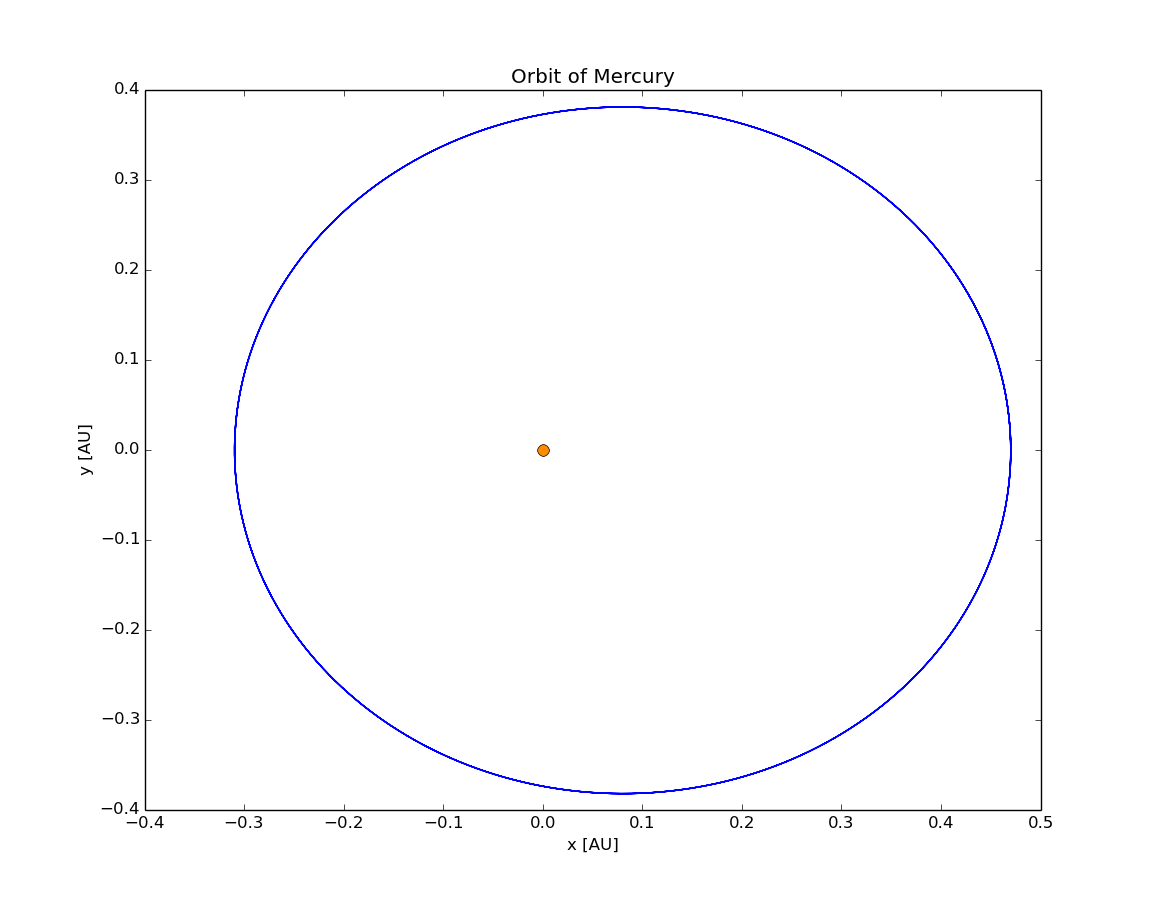
\includegraphics[width = \linewidth]{lab1q5p1.png}
\caption{Orbital position of Mercury over the course of one Earth year. The yellow dot marks the Sun's position.}
\label{fig:q5p1}
\end{figure}

\begin{figure}[H]
\centering
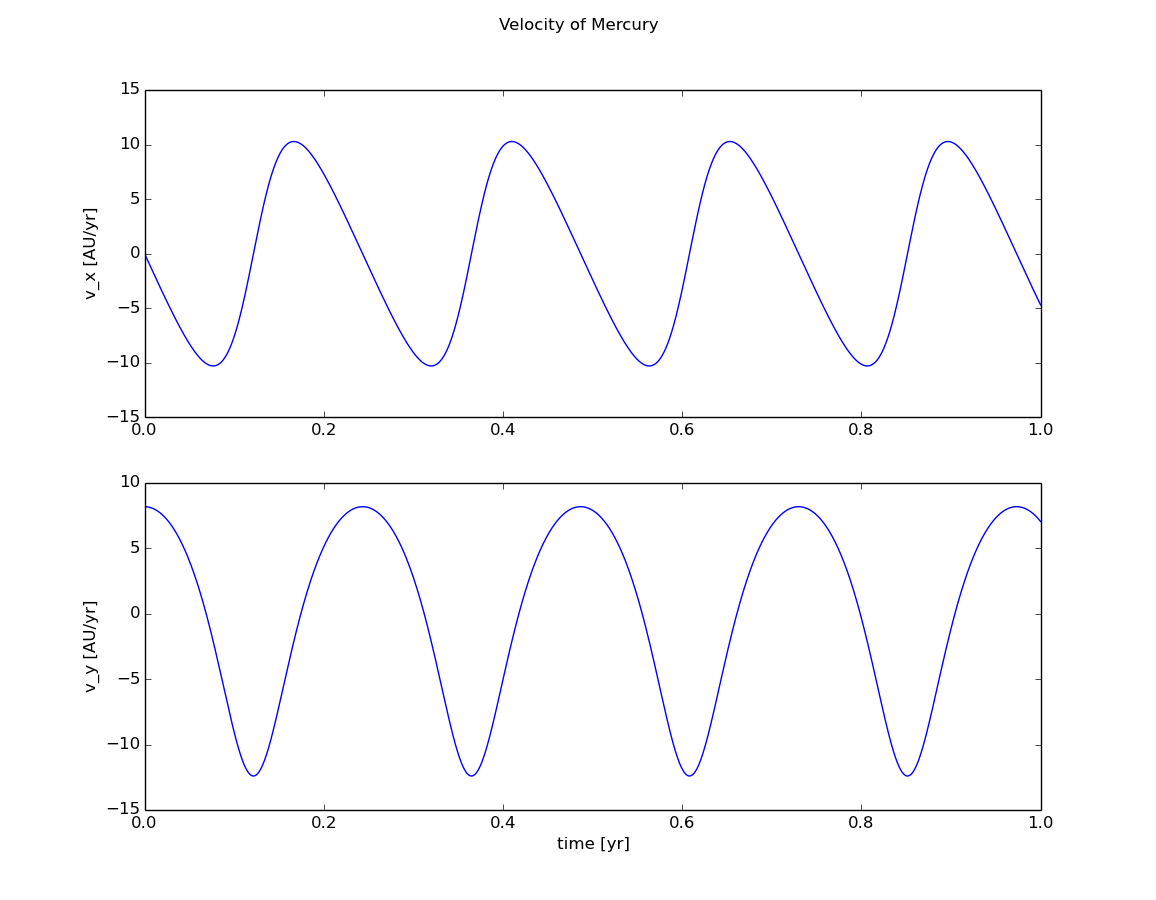
\includegraphics[width = \linewidth]{lab1q5p2.png}
\caption{Velocity of Mercury in each dimension over the course of one Earth year.}
\label{fig:q5p2}
\end{figure}

\section{Question 6 Plot}

\begin{figure}[H]
\centering
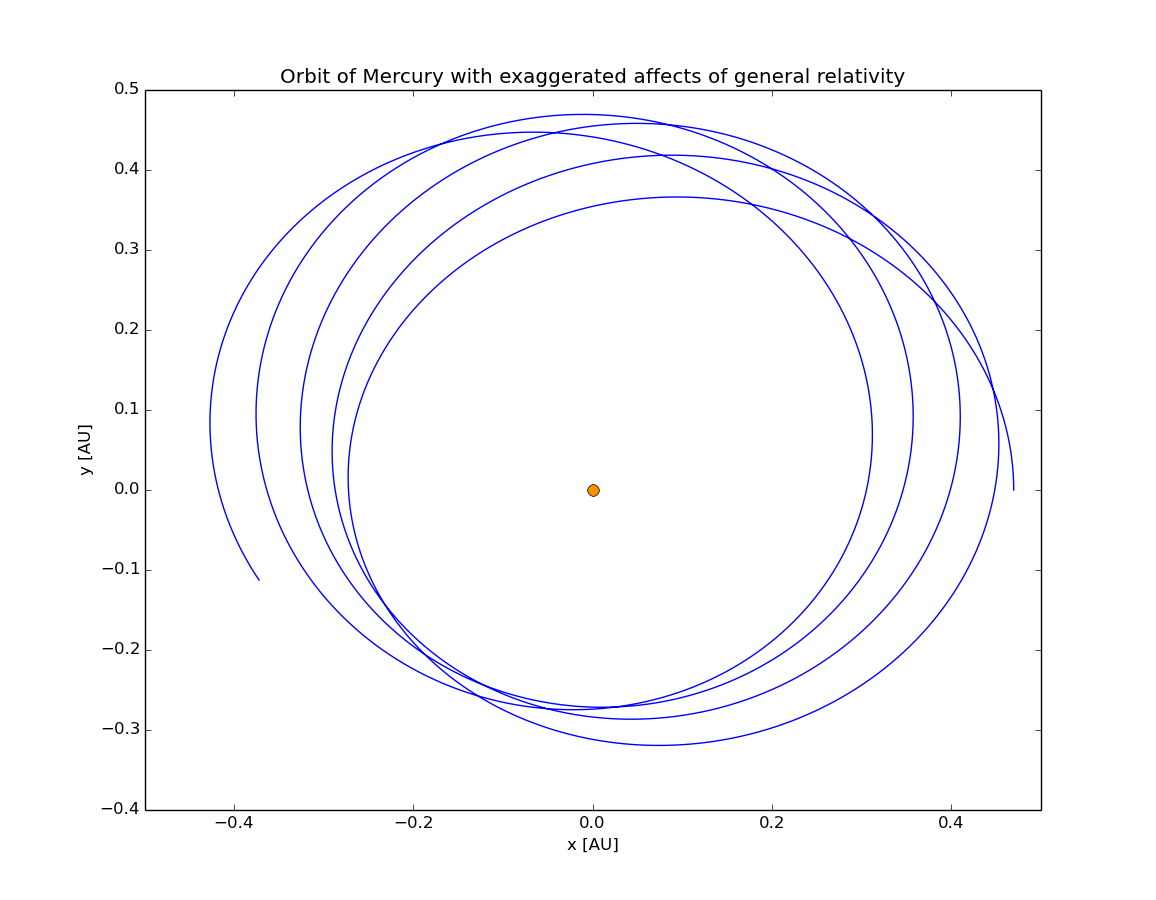
\includegraphics[width = \linewidth]{lab1q6.png}
\caption{Orbital position of Mercury over the course of one Earth year with exaggerated affects of general relativity ($\alpha = 0.01\, AU^2$). The yellow dot marks the Sun's position.}
\label{fig:q6}
\end{figure}

\section{Question 7 Plot}

\begin{figure}[H]
\centering
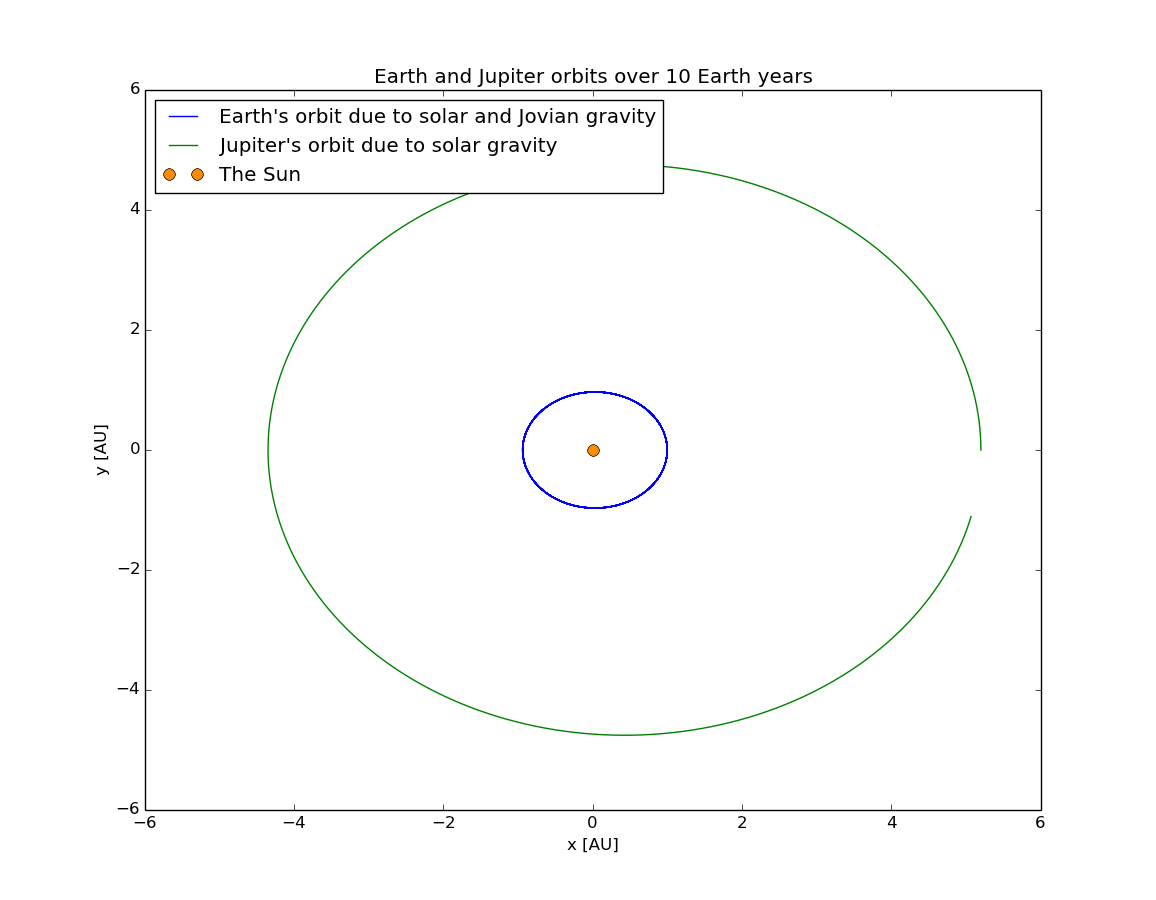
\includegraphics[width = \linewidth]{lab1q7.png}
\caption{Orbital position of the Earth and Jupiter over the course of 10 Earth years, with the mass of Jupiter as $M_{jup} = 1\e{-3}\, M_{sun}$.}
\label{fig:q7}
\end{figure}

\section{Question 8 Plot}

\begin{figure}[H]
\centering
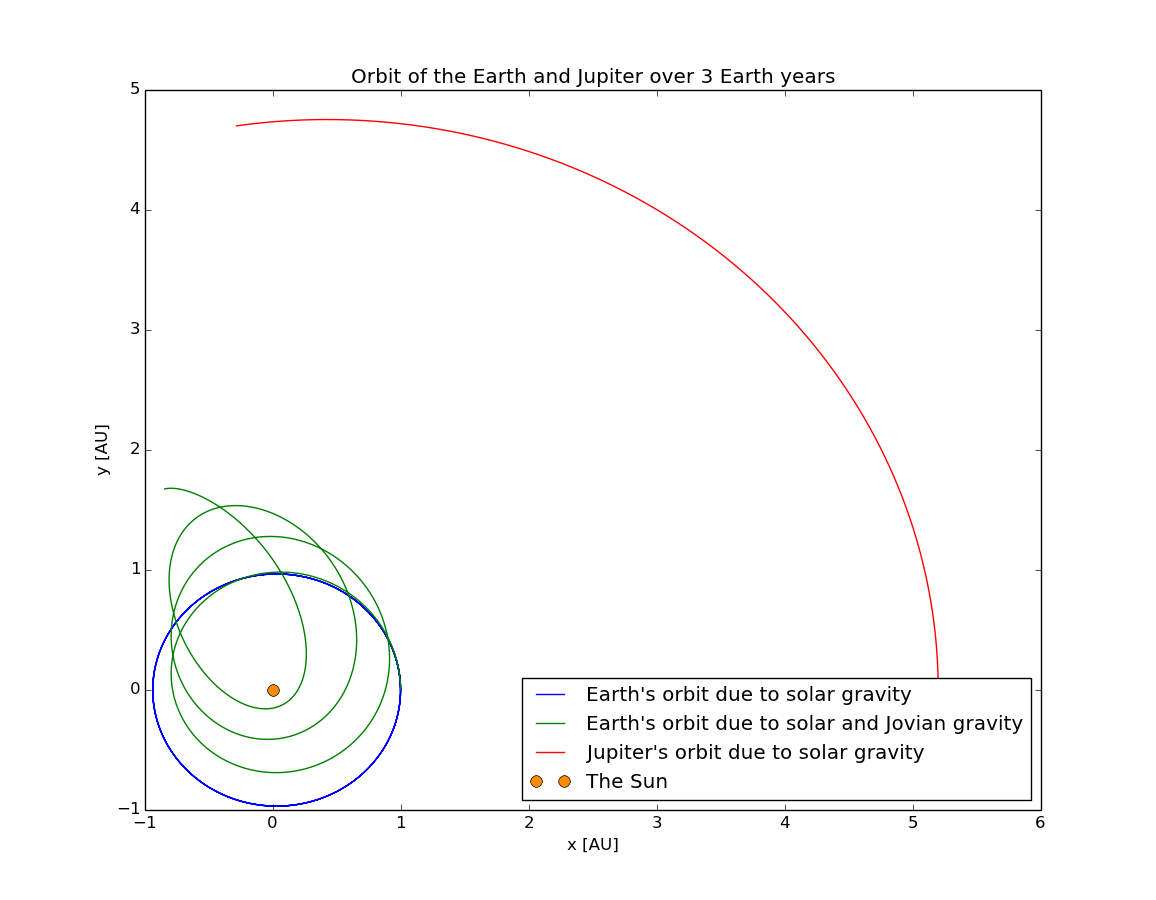
\includegraphics[width = \linewidth]{lab1q8.png}
\caption{Orbital position of the Earth and Jupiter over the course of 3 Earth years, with the mass of Jupiter as $M_{jup} = 1\, M_{sun}$.}
\label{fig:q8}
\end{figure}

\end{document}